\chapter{Anytime and Efficient Multi-agent Coordination for Disaster Response}\label{chap:contrib1}

In this chapter, we begin by presenting the \emph{Coalition Formation with improved
Look-Ahead} (CFLA2), an extension of the CFLA algorithm (Section \ref{sec:cfla}). Despite
having better performance, CFLA2 keeps the design limitations of CFLA, which is why we
propose the novel CTS algorithm in Section \ref{sec:cts}. We compare CTS with CFLA and
CFLA2 in Section \ref{sec:tests}, and evaluate its performance with a well-established
testbed in Section \ref{sec:robotests}.

\section{Coalition Formation with Improved Look-ahead}

We give a more detailed formulation of Phase $2$ in Section \ref{sec:cfla2b}, and describe
an improved Phase $3$ in Section \ref{sec:cfla3b}, which constitutes the novelty of CFLA2.
Finally, we list the design limitations of both CFLA and CFLA2 in Section \ref{sec:an1}.

\subsection{Forming Coalitions with Legal Agent Allocations}\label{sec:cfla2b}

To minimise both the size of $C^*_v$ and the time at which it completes task $v$,
Algorithm \ref{algo:ecf2} iterates from the smallest to the largest possible coalition
size (line $5$), and through all possible coalitions of each size (line $6$). When the
procedure finds a coalition $C$ that can complete $v$ by its deadline $\gamma_v$ (line $7$),
then $|C|$ is the minimum size of the coalitions that can complete $v$. Hence, $C^*_v$ is
identified among the coalitions with size $|C|$ (lines $8 - 11$). The summations at
lines $7 - 8$ capture the workload done by the coalition allocations defined from the
asynchronous arrivals (Section \ref{sec:constraints}) of the agents in $C$ to the location
of $v$.
\clearpage

Unlike the original formulation (Algorithm \ref{algo:ecf}), Algorithm \ref{algo:ecf2}
clarifies that the minimum coalition size is determined by iterating through
subsets of the combinations\footnote{To date, the most efficient technique to enumerate
all such combinations is the Gray binary code \cite[Section $7.2.1.1$]{knuth2005}.} of
$A^t_v$, which is the set of free agents that at time $t$ can reach $v$ by $\gamma_v$.

\begin{algorithm}[t]
    \DontPrintSemicolon
    \KwIn{task $v$, a set of legal agent allocations $\text{Leg}_t$}
    $A_v^t \gets $ define from $\text{Leg}_t$ the agents that can reach $v$ at $t$ by
    $\gamma_v$\;
    $C^*_v \gets \emptyset$ \Comment*[h]{\small the ECF coalition}\;
    $t^*_v \gets \gamma_v + 1$ \Comment*[h]{\small time at which $C^*_v$ completes $v$}\;
    $i \gets 1$\;
    \While{$i \leq |A^t_v| \text{\normalfont and } C_v^* = \emptyset$}{
        \For{\normalfont$C \in$ all combinations of $i$ agents in $A^t_v$}{
            \If{ $\sum_{\alloc{C}{t'} \in \Gamma_v \text{, } C' \subseteq C \text{, } t' \in \left[ t, \gamma_v \right]}
                u(C, v) \geq w_v$ }{
                $t_{minmax} \gets \min_{t_{max}} \left( w_v -
                    \sum_{\alloc{C}{t'} \in \Gamma_v \text{, } C' \subseteq C \text{, } t' \in \left[ t, t_{max} \right]}
                u(C, v) \right)$\;
                \If { $t_{minmax} < t^*_v $ }{
                    $t^*_v \gets t_{minmax}$\;
                    $C^*_v \gets C$\;
                }
            }
        }

        $i \gets i + 1$\;
    }
    \Return $C^*_v$\;
    \caption{\textsf{ECF} (more detailed Phase $2$ of CFLA2)\label{algo:ecf2}}
\end{algorithm}

\subsection{More Effective Task Degrees}\label{sec:cfla3b}

\begin{algorithm}[t]
    \DontPrintSemicolon
    \KwIn{task $v$, its ECF coalition $C^*_v$, the set of all agent allocations $T$}
    $\delta_v \gets 0$ \Comment*[h]{\small the degree of task $v$}\;
    $f_v \gets $ time at which $C^*_v$ completes $v$\;
    \For{$v_2 \in V_{unc} \setminus \{ v \}$}{
        \If{$d_{v_2} \geq \gamma_v$}{
            $A_{free}^{f_v} \gets$ agents that are free at $f_v$ \Comment*[h]{\small
            derived from $C^*_v$ and $T$}\;
            $A^{d_{v_2}} \gets$ select from $A_{free}^{f_v}$ the agents that can reach
            $v_2$ by $d_{v_2}$ \;
            $i \gets 1$\;
            \While{$i \leq |A^{d_{v_2}}|$}{
                \For{\normalfont$C \in$ all combinations of $i$ agents in $A^{d_{v_2}}$}{
                    \Comment*[h]{\small if $C$ can complete $v_2$}\;
                    \If{ $\sum_{\alloc{C'}{t} \in \Gamma_v \text{, } C' \subseteq C \text{, } t \in \left[ f_v, d_{v_2}
                        \right]} u(C, v) \geq w_v$ }{
                        $\delta_v \gets \delta_v + 1 + (1 - \eta_{v_2})$\;
                        $i \gets |A^{d_{v_2}}|$ \Comment*[h]{\small break
                        external loop too}\;
                        \Break
                    }
                }

                $i \gets i + 1$\;
            }
        }
    }
    \Return $\delta_v$\;
    \caption{\textsf{lookAhead} (improved Phase $3$ of CFLA2)\label{algo:la2}}
\end{algorithm}

Algorithm \ref{algo:la2} differs from the original look-ahead phase (Algorithm
\ref{algo:la2}) in $2$ points. First, it only considers uncompleted tasks that have a
deadline greater or equal to $\gamma_v$ (line $4$), which prevents from counting tasks that can
be completed before the completion of $v$.
This is because, as defined in Section \ref{sec:cfla_gen}, $\delta_v$ must represent the
number of tasks that can be completed only after the completion of $v$.
Second, at line $11$, $\delta_v$ is not just incremented by $1$, but also by $1 -
\eta_{v_2}$, where $\eta_{v_2}$ is the rescaling\footnote{Also known as min-max scaling or
min-max normalisation.} of $w_{v_2}$ to the range $[w_{min}, w_{max}]$, with $w_{min}$ and
$w_{max}$ being respectively the minimum and maximum task workloads:
$\eta_{v_2} = \left( w_{v_2} - w_{min} \right) / \left(w_{max} - w_{min} \right)$.
Hence, $\delta_v$ is also a measure of how much total workload remains after the
completion of $v$. Maximising $\delta_v$ (line $12$ in Algorithm \ref{algo:cfla}) leads to
the remaining tasks with the smallest workloads, which increases the probability of
completing more.

\subsection{Analysis and Discussion}\label{sec:an1}

Algorithm \ref{algo:alloc} iterates through all free agents and uncompleted tasks.
Assuming that line $4$ requires constant time, the time complexity is $\bar{a} = O(|A|
\cdot |V|)$.

Algorithm \ref{algo:ecf2} iterates (line $5$) from coalition size $1$ to $|A^t_v|$, where
$A^t_v$ is the set of agents that can reach task $v$ at time $t$. This needs $O(|A|)$
time in case $A^t_v = A$. For each $i \leq |A^t_v|$, examining the set of all possible
coalitions of size $i$ (line $6$) requires $O(2^{|A|})$ time. Assuming that line $8$
takes $O(\tmax)$ time, the total time complexity is $\bar{b} = O(|A| \cdot 2^{|A|}
\cdot \tmax)$.

Algorithm \ref{algo:la2} iterates through all uncompleted tasks, which requires $O(|V|)$
time, while line $8$ is computationally identical to line $5$ in Algorithm \ref{algo:ecf2}.
Hence, the time complexity is $\bar{c} = O(|V| \cdot 2^{|A|})$.

Algorithms \ref{algo:ecf} and \ref{algo:la} have the same time complexity of Algorithms
\ref{algo:ecf2} and \ref{algo:la2}, respectively. As it uses Phases $1 - 3$, Algorithm
\ref{algo:cfla} has a time complexity of:
\begin{equation}
    O \left(\tmax \cdot \left( \bar{a} + |V| \cdot (\bar{b} + \bar{c}) \right)
    \right) = O \left( \left(\tmax \cdot |V|\right)^2 \cdot 2^{|A|} \right)
\end{equation}
Therefore, the runtime of CFLA2 is quadratic in the number of tasks and exponential in the
number of agents, which makes it not suitable for systems with limited resources or
real-time applications (Section \ref{sec:pstat}). Other limitations are:
\begin{enumerate}
    \item
        It can allocate at most one task per time \cite[Section $7$]{ramchurn2010cfstp}.
        More formally, at each time $t$, the best-case guarantee of CFLA2 is to find a
        solution with degree $k = 1$;
    \item
        In general, greedily allocating a task with the highest degree now does not ensure
        to allocate all uncompleted tasks in future. This is particularly relevant in
        dynamic environments, where there is no certainty of having further tasks to be
        completed (Section \ref{sec:pstat});
    \item
        The more tasks can be grouped by degree, the more the look-ahead technique
        becomes a costly random choice. In other words, at time $t$, if some tasks $V^{'}
        \subseteq V$ have all maximum degree, then Algorithm \ref{algo:cfla} selects $v^*$
        randomly from $V^{'}$. Hence, the larger $V^{'}$ is, the less relevant Algorithm
        \ref{algo:la2} becomes;
    \item
        In Algorithm \ref{algo:cfla}, all tasks have the same weight. That is, tasks with
        earlier deadlines may not be allocated before tasks with later deadlines. This is
        independent of the order in which uncompleted tasks are elaborated (line $9$),
        since the computation of $\delta_{max}$ (line $11$) would not be affected.
\end{enumerate}

To overcome the limitations of CFLA2, in the next section we present a CFSTP algorithm
that is anytime, efficient and with convergence guarantee, both in static and dynamic
environments.

\section{Cluster-based Task Scheduling}\label{sec:cts}

\emph{Cluster-based Task Scheduling} (CTS) algorithm operates at the agent level, rather
than at the coalition level. Using the terminology of \cite{gerkey2004}, we can say that
it decomposes a Single-Task Multi-Robot problem into a sequence of Single-Task
Single-Robot problems. It is divided into the following two phases:
\begin{enumerate}
    \item For each free agent $a$, associate $a$ with an uncompleted task $v$ such that
        $v$ is the closest to $a$ and deadline $\gamma_v$ is minimum;
    \item For each uncompleted task $v$, allocate $v$ to a coalition $C$ such that $|C|$
        is minimum and each agent $a \in C$ has been associated with $v$ in Phase $1$.
\end{enumerate}
Algorithm \ref{algo:getTask} is used in Phase $1$, while Algorithm \ref{algo:cts} enacts
both phases. We describe them in Sections \ref{sec:getTask} and
\ref{sec:cts2}, respectively.

\subsection{Selecting the Best Task for Each Agent}\label{sec:getTask}

\begin{algorithm}[t]
    \DontPrintSemicolon
    \KwIn{time $t$, agent $a$}
    $v_a^t \gets $ (\textsc{nil}, \textsc{nil}) \Comment*[h]{\small array in which
    $v_a^t[0]$ (resp. $v_a^t[1]$) is the unallocated (resp. allocated but still
    uncompleted) task allocable to agent $a$ at time $t$}\;
    $t_{min} \gets (\tmax + 1, \tmax + 1)$ \Comment*[h]{\small array in which
$t_{min}[0]$ (resp. $t_{min}[1]$) defines the time units required by agent $a$
to reach $v_a^t[0]$
(resp. $v_a^t[1]$)}\;
    $t_{min} \gets (\tmax + 1, \tmax + 1)$ \Comment*[h]{\small array in which
    $t_{min}[0]$ (resp. $t_{min}[1]$) is the deadline of $v_a^t[0]$ (resp.
    $v_a^t[1]$)}\;
    \For(\Comment*[h]{\small for each uncompleted task}){$v \in V$}{
        $i \gets 0$ \Comment*[h]{\small $v$ is unallocated}\;
        \If{\normalfont other agents are travelling to or working on $v$}{
            $i \gets 1$ \Comment*[h]{\small $v$ is allocated but still uncompleted}\;
        }
        $t_{arr} \gets t + \rho(a, l_a^t, l_v)$\;
        \If(\Comment*[h]{\small $a$ can reach $v$ by $\gamma_v$ and $v$ is the closest to
            $a$}){\normalfont $t_{arr} \leq \gamma_v$ and $t_{arr} < t_{min}[i]$ and $\gamma_v < t_{min}[i]$}{
            $v_a^t[i] \gets v$\;
            $t_{min}[i] \gets t_{arr}$\;
            $t_{min}[i] \gets \gamma_v$\;
        }
    }
    \If(\Comment*[h]{\small prioritise unallocated tasks}){$v^t_a[0] \neq$
        \textsc{\normalfont nil}}{
        \Return{$v^t_a[0]$}\;
    }
    \Return{$v^t_a[1]$}\;
    \caption{\textsf{getTaskAllocableToAgent} (used in Phase $1$ of CTS)\label{algo:getTask}}
\end{algorithm}

Given a time $t$ and an agent $a$, Algorithm \ref{algo:getTask} returns the uncompleted
task $v$ that is allocable, the most urgent and closest to $a$. By \emph{allocable} we
mean that $a$ can reach $v$ before deadline $\gamma_v$, while \emph{most urgent} means
that $v$ has the earliest deadline. The algorithm prioritises unallocated tasks, that is,
it first tries to find a task to which no agents are travelling, and on which no agents
are working ($v_a^t[0]$). Otherwise, it returns an already allocated but still
uncompleted task such that $a$ can reach it and contribute to its completion ($v_a^t[1]$).
This ensures that $a$ becomes free only when no other tasks are uncompleted and allocable
to $a$ and.

\subsection{Overall Procedure of CTS}\label{sec:cts2}

\begin{algorithm}
    \DontPrintSemicolon
    \KwIn{tasks $V$, task demands $(\gamma_v, w_v)_{v \in V}$, agents $A$, locations $L$,
    travel function $\rho$, coalition value function $u$}
    $t \gets 0$\;
    $\Gamma' \gets \emptyset$
    \Comment*[h]{\small the solution to return (a set of coalition allocations)}\;
    $V_{allocable} \gets \emptyset$ \Comment*[h]{\small allocable tasks}\;
    \Repeat{\normalfont $V = \emptyset$ or $t > \tmax$ or all agents are free}{
        \For(\Comment*[h]{\small Phase 1: satisfy spatial constraints}\label{algo:phase1}){$a \in A$}{
            \eIf{$a \in A^t_{free}$}{
                $v \gets $ \textsf{getTaskAllocableToAgent($t$, $a$)} \Comment*[h]{\small
                Algorithm \ref{algo:getTask}}\;
                \If{$v \neq \text{\textsc{nil}}$}{
                    \If{$v \not\in V_{allocable}$}{
                        $V_{allocable} \gets V_{allocable} \cup \{v\}$\;
                    }
                    $A^t_v \gets A^t_v \cup \{ a \}$\;
                }
                }{
                Update $a$'s location\;
                \If{\normalfont $a$ reached the task $v$ to which it was assigned}{
                    Set $a$'s status to \emph{working on $v$}\;
                }
            }
        }
        \For(\Comment*[h]{\small Phase 2: satisfy temporal constraints}\label{algo:phase2}){$v \in V$}{
            $C_v^t \gets$ all agents working on $v$ at time $t$\;
            \If{$v \in V_{allocable}$}{
                $\Pi^t_v \gets$ list of all agents in $A^t_v$ sorted by arrival time to
                $l_v$\;
                $C^* \gets \emptyset$\;
                \For{$i \gets 1$ \KwTo $|\Pi^t_v|$}{
                    $C^* \gets $ first $i$ agents in $\Pi^t_v$\;
                    $\lambda_i \gets $ arrival time to $l_v$ of the $i$-th agent
                    in $\Pi^t_v$\;
                    \eIf{$i + 1 \leq |\Pi^t_v|$}{
                        $\lambda_{i+1} \gets $ arrival time to $l_v$ of the $(i+1)$-th
                        agent in $\Pi^t_v$\;
                    }{
                        $\lambda_{i+1} \gets \gamma_v$\;
                    }
                    $\varphi_v \gets \varphi_v + (\lambda_{i+1} - \lambda_i)
                    \cdot u(C^* \cup C^t_v, v)$ \Comment*[h]{\small $w_v$ done at
                    $\lambda_{i+1}$}\;
                    \If { $(\gamma_v - \lambda_{i+1}) \cdot u(C^*, v) \geq w_v -
                        \varphi_v$ }{
                        \Break \Comment*[h]{\small $C^*$ is the minimum coalition
                        to complete $v$}
                    }
                }
                $T_v = \bigcup_{a \in C^*} \left\{ \alloc{a}{\lambda_a} \right\}$
                \Comment*[h]{\small $\lambda_a$ is $a$'s arrival time to $l_v$}\;
                $\Gamma' \gets \Gamma' \cup \Gamma(T_v, t)$
                \Comment*[h]{\small add $\Gamma(T_v, t)$ (Section \ref{sec:ca}) to
                $\Gamma'$}\;
                $V_{allocable} \gets V_{allocable} \setminus \{v\}$\;
            }
            \If{$C_v^t \neq \emptyset$}{
                $w_v \gets w_v - u(C_v^t, v)$\;
                \If{$w_v \leq 0$}{
                    Set free all agents in $C_v^t$\;
                    $V \gets V \setminus \{v\}$\;
                }
            }
        }
        $t \gets t + 1$\;
    }
    \Return $\Gamma'$\;
    \caption{Overall procedure of \textsf{CTS} (Phases $1$ and $2$)\label{algo:cts}}
\end{algorithm}

The overall procedure is described in Algorithm \ref{algo:cts}. The \textsf{repeat-until}
loop is the same as CFLA2, to preserve the anytime property. Phases $1$ and $2$ are
represented respectively by the loops at lines \ref{algo:phase1} and \ref{algo:phase2}.

Phase $1$ loops through all agents (line $5$). Here, an agent $a$ may either be free or
reaching a task location. In the first case (line $6$), if an uncompleted task $v$ can be
allocated to $a$ (lines $7 - 8$), then $v$ is flagged as allocable (line $9$) and $a$ is
added to the set of agents $A^t_v$ to which $v$ could be allocated at time $t$ (line
$11$). In the second case (line $12$), $a$ is travelling to a task $v$, hence its location
is updated (line $13$) and, if it reached $v$, it is set to \emph{working on $v$} (lines
$14 - 15$).

Phase $2$ visits each uncompleted task $v$ (line $16$). If $v$ is allocable (line $18$)
then it is allocated to the smallest coalition of agents in $A^t_v$ (defined in Phase $1$)
that can complete it (lines $19 - 33$). In particular, at line $28$, $\varphi_v$ is the
amount of work done by all the coalitions formed after the arrival to the location of $v$
of the first $i$ agents in $\Pi_v^t$ (defined at line $19$).
After that, if there are agents working on $v$ (line $34$), its workload $w_v$ is
decreased accordingly (line $35$). If $w_v$ drops to zero or below, then $v$ has been
completed (lines $36 - 38$). The algorithm stops (line $40$) when all the tasks have been
completed, or the maximum problem time is expired, or no other tasks are allocable and
uncompleted (Section \ref{sec:getTask}).
\clearpage

The spatial constraints (Equations \ref{eq:s1} and \ref{eq:s2}) are satisfied by executing
Algorithm \ref{algo:getTask} only on free agents (line $7$), while the temporal
constraints (Equation \ref{eq:t1}) are satisfied by allocating a task $v$ to a coalition
$C$ only when $C$ has minimum size and can complete $v$ by deadline $\gamma_v$.

\subsection{Analysis and Discussion}\label{sec:nova}

The approach of CTS transforms the CFSTP from a $1 - k$ task allocation to a series of $1
- 1$ task allocations. In other words, instead of allocating each task to a coalition of
$k$ agents, coalitions are formed by \emph{clustering} or grouping agents based on the
closest and most urgent tasks. This is an eligibility criterion: unlike CFLA2, CTS
exploits the distances between agents and tasks and the speeds of agents to reduce the
time needed to define coalition allocations.
Algorithm \ref{algo:getTask} runs in $\bar{a} = O(|V|)$ time, assuming that the
operation at line $8$ has constant time. In Algorithm \ref{algo:cts}, the time
complexity of Phase $1$ is $O(|A| \cdot \bar{a}) = O(|A| \cdot |V|)$, while Phase $2$
runs in $O(|V| \cdot |A| \log |A|)$ because: in the worst case, $A^t_v = A$ and
line $19$ sorts $A$ in $\Omega(|A|\cdot\log|A|)$ time using any sorting algorithm based on
comparisons \cite{cormen2009}; the loop at line $21$ runs in $O({|A|})$ time.  Since the
\textsf{repeat-until} loop is executed at most $\tmax$ times, the time complexity of
Algorithm \ref{algo:cts} is:
\begin{equation}\label{eq:comp1}
    O \left( \tmax \cdot |V| \cdot |A| \log |A| \right)
\end{equation}
If both phases are executed in parallel, the time complexity is reduced to:
\begin{equation}\label{eq:comp2}
    \Omega \left( \tmax \cdot \left( |V| + |A| \log |A| \right) \right)
\end{equation}
CTS does not have the limitations of CFLA2 (Section \ref{sec:an1}) because:
\begin{enumerate}
    \item It can allocate more than one task per time. More formally, at each time $t$, if
        one or more tasks are allocable, CTS finds a solution with degree $1 \leq k \leq
        |A|$;
    \item It runs in polynomial time and does not use a look-ahead technique. Thus, it is
        efficient and can be used in dynamic environments.
\end{enumerate}

%The following theorem is based on the definitions given in Section \ref{sec:cfstp}.

\begin{theorem}\label{teo:correctness}
    CTS is guaranteed to find feasible coalition allocations.
\end{theorem}
\begin{proof}
    We prove by induction on time $t$.

    At $t = 0$, Phase $1$ of Algorithm \ref{algo:cts} selects a task $v$ for each agent
    $a$ such that $v$ is allocable, the most urgent and closest to $a$ (Section
    \ref{sec:getTask}). This implies that the agent allocation $\alloc{a}{0}$ is legal
    (Section \ref{sec:constraints}). Then, Phase $2$ (Section \ref{sec:cts2}) allocates
    $v$ to $a$ only if it exists a coalition $C$ such that $|C|$ is minimum,
    $\alloc{C}{0}$ is feasible (Section \ref{sec:constraints}) and $a \in C$.

    At $t > 0$, for each agent $a$, there are $2$ possible cases: a task $v$ has been
    allocated to $a$ at time $t' < t$, or $a$ is free (i.e., idle). In the first case, $a$
    is either reaching or working on $v$ (lines $12 - 15$ in Algorithm \ref{algo:cts}),
    hence $\alloc{a}{t}$ is legal and $\alloc{C}{t}$ is feasible, where $a \in C$. In the
    second case, $a$ is either at its initial location or at the location of a task on
    which it finished working at time $t' < t$. Thus, as in the base case, if it exists a
    coalition $C$ and a task $v$ such that $|C|$ is minimum, $\alloc{C}{t}$ is feasible
    and $a \in C$, then $v$ is allocated to $a$.
\end{proof}

\begin{theorem}\label{teo:convergence}
    CTS converges to a solution, if it exists.
\end{theorem}
\begin{proof}
    First we show that CTS always finds a solution, then that it terminates.

    \emph{Finding a solution}.
    From Theorem \ref{teo:correctness} it follows that the coalition allocations in the
    set $\Gamma(T_v, t)$ at line $32$ of Algorithm \ref{algo:cts} are feasible. That is,
    they satisfy all constraints (Section \ref{sec:constraints}).
    Since $\Gamma(T_v, t)$ also defines the minimum number of agents necessary to complete
    task $v$ (line $29$ of Algorithm \ref{algo:cts}), it is a solution to $v$, thus it has
    degree $k = 1$.
    Therefore, if $V_{allocable} \neq \emptyset$ at some time $t \leq \tmax$, then
    $\Gamma'$ (line $41$) has degree $k \geq 1$.

    \emph{Termination}.
    Algorithm \ref{algo:getTask} iterates exactly once over a finite set of uncompleted
    tasks, while the \textsf{repeat-until} loop of Algorithm \ref{algo:cts} is executed at
    most $\tmax$ times.
\end{proof}
In finding a solution to a task $v$, CTS defines a coalition of minimum size among the
agents that are closest to $l_v$. To make a comparison with an exhaustive search, this
means that CTS stops at the first valid solution.
\iffalse
Let $S_v$ be the set of solutions for $v$. In general, $x$ may not be optimal, but if $S_v
\neq \emptyset$, then $x \in S_v$.
\fi

The counterexample given by Limitation $2$ in Section \ref{sec:an1} does not allow to
prove the convergence of CFLA and CFLA2 in dynamic environments. Since no current
algorithm that solves the CFSTP is simultaneously anytime, efficient and with convergence
guarantee (Section \ref{chap2:limitations}), CTS is the first of its kind.

\section{Comparison Tests}\label{sec:tests}

We implemented CFLA, CFLA2 and CTS in
Java\footnote{\url{https://doi.org/10.5281/zenodo.4320671}}, and replicated the
experimental setup of \cite{ramchurn2010cfstp} because we wanted to evaluate how well
CFLA2 and CTS perform in settings where the look-ahead technique is highly effective. For
each test configuration, we solved $100$ random CFSTP instances and plotted the average
and standard deviation of: percentage of completed tasks; agent travel time
(Section \ref{sec:defs}); \emph{task completion time}, or the time at which a task has no
workload left; \emph{problem completion time}, or the time at which no other tasks can be
allocated.

\subsection{Setup}

Let $\mathcal{U}(l, u)$ and $\mathcal{U}^I(l, u)$ be respectively a uniform real
distribution and a uniform integer distribution with lower bound $l$ and upper bond $u$.
Our parameters are defined as follows:
\begin{itemize}
    \item All agents have the same speed. Their initial locations are randomly chosen on a
        $50 \times 50$ grid, where the travel time of agent $a$ between two locations is
        given by the Manhattan distance (i.e., the taxicab metric or $\ell_1$ norm)
        divided by the speed of $a$;
    \item Tasks are fixed to $300$, while agents range from $2$ to $40$, in intervals of
        $2$ between $2$ and $20$ agents, and in intervals of $5$ between $20$ and $40$
        agents;
    \item The coalition values are defined as $u(C, v) = |C| \cdot k$, where $k \sim
        \mathcal{U}(1, 2)$. Hence, coalition values depend only on the number of agents
        involved, and all tasks have the same difficulty;
    \item Deadlines $\gamma_v \sim \mathcal{U}^I(5,600)$ and workloads $w_v \sim
        \mathcal{U}^I(10, 50)$.
\end{itemize}

Unlike \cite{ramchurn2010cfstp}, we set the number of maximum agents to $40$ instead of
$20$, because it allows in this setup to complete all tasks in some instances. We did not
perform a comparison on larger instances because of the runtime of CFLA and CFLA2: on
commodity hardware, CTS takes seconds to solve instances with thousands of agents and
tasks, while CFLA and CFLA2 take days. Consequently, the purpose of this section is to
highlight the performance of CTS using CFLA and CFLA2 as baselines. We evaluate the
scalability of CTS in Chapter \ref{chap:contrib2}.

\subsection{Results}

\begin{figure}[t]
    \centering
    \begin{adjustbox}{width=\textwidth}
        \begin{tikzpicture}
    \begin{groupplot}[%
            group style={group size=2 by 2, vertical sep=1.75cm, horizontal sep=1.75cm},
            grid=both,
            grid style={line width=.1pt, draw=gray!10},
            major grid style={line width=.2pt,draw=gray!50},
            minor tick num=5,
            ymin=0,
            legend style={/tikz/every even column/.append style={column sep=1em}, legend
            columns=-1, at={(0.26,2.55)}, anchor=north east},
            cycle list name=exotic2]

        \nextgroupplot[xlabel=Number of agents,ylabel=Completed tasks ($\%$), title=(a)]

        % NOTE: written +- but it actually is -+

        % CFLA
        \addplot+[error bars/.cd, y dir=both, y explicit,%
        error bar style = {thick}] coordinates {%
            (2 , 27.24) +- (1.91, 2.09)
            (4 , 42.01) +- (4.01, 3.99)
            (6 , 51.24) +- (4.24, 4.10)
            (8 , 57.94) +- (4.94, 4.06)
            (10, 61.87) +- (3.87, 4.80)
            (12, 65.14) +- (4.14, 7.52)
            (14, 67.11) +- (5.44, 4.22)
            (16, 68.77) +- (4.10, 5.23)
            (18, 69.73) +- (6.07, 5.60)
            (20, 70.67) +- (7.00, 5.00)
            (25, 71.35) +- (4.68, 5.65)
            (30, 70.97) +- (5.97, 4.70)
            (35, 71.19) +- (4.53, 5.14)
            (40, 70.79) +- (5.46, 5.54)
        };

        % CFLAP
        \addplot+[error bars/.cd, y dir=both, y explicit,%
        error bar style = {thick}] coordinates {%
            (2 , 23.68) +- (2.68, 2.98)
            (4 , 43.76) +- (3.76, 4.24)
            (6 , 60.55) +- (5.22, 3.45)
            (8 , 74.30) +- (5.63, 3.70)
            (10, 83.59) +- (5.25, 4.75)
            (12, 87.43) +- (5.76, 4.24)
            (14, 87.94) +- (5.60, 4.40)
            (16, 89.10) +- (4.10, 5.23)
            (18, 89.10) +- (4.10, 3.90)
            (20, 89.34) +- (7.67, 3.66)
            (25, 89.30) +- (3.96, 4.37)
            (30, 88.94) +- (4.27, 3.73)
            (35, 89.46) +- (4.46, 4.21)
            (40, 89.27) +- (4.27, 2.73)
        };

        % CTS
        \addplot+[error bars/.cd, y dir=both, y explicit,%
        error bar style = {thick}] coordinates {%
            (2 ,  9.41) +- (8.74, 5.26)
            (4 , 26.37) +- (6.04, 2.63)
            (6 , 39.33) +- (3.99, 3.67)
            (8 , 52.25) +- (4.59, 3.75)
            (10, 63.88) +- (5.88, 5.78)
            (12, 74.73) +- (4.06, 4.27)
            (14, 82.38) +- (5.05, 4.28)
            (16, 86.94) +- (7.94, 5.39)
            (18, 89.49) +- (6.15, 5.51)
            (20, 91.99) +- (6.32, 4.01)
            (25, 95.18) +- (5.51, 3.15)
            (30, 96.19) +- (5.19, 2.81)
            (35, 97.29) +- (4.62, 2.71)
            (40, 98.15) +- (2.48, 1.85)
        };

        \nextgroupplot[title=(b),xlabel=Number of agents,ylabel=Agent travel time]

        % CFLA
        \addplot+[error bars/.cd, y dir=both, y explicit,%
        error bar style = {thick}] coordinates {%
            (2 , 31.67) +- (4.32, 6.06)
            (4 , 32.14) +- (4.36, 3.57)
            (6 , 32.34) +- (3.69, 4.26)
            (8 , 32.62) +- (3.19, 3.43)
            (10, 32.59) +- (2.96, 3.11)
            (12, 32.95) +- (3.18, 3.17)
            (14, 33.06) +- (3.16, 2.63)
            (16, 32.86) +- (2.67, 2.83)
            (18, 32.54) +- (3.83, 4.71)
            (20, 32.83) +- (2.46, 2.77)
            (25, 32.66) +- (3.10, 3.09)
            (30, 32.50) +- (3.89, 3.20)
            (35, 32.25) +- (2.50, 2.63)
            (40, 32.34) +- (3.20, 2.79)
        };

        % CFLAP
        \addplot+[error bars/.cd, y dir=both, y explicit,%
        error bar style = {thick}] coordinates {%
            (2 , 14.87) +- (2.33, 2.78)
            (4 , 17.64) +- (2.98, 2.71)
            (6 , 19.96) +- (2.43, 2.91)
            (8 , 22.26) +- (2.05, 1.95)
            (10, 25.13) +- (3.62, 4.27)
            (12, 29.14) +- (4.97, 3.44)
            (14, 31.00) +- (2.76, 2.66)
            (16, 31.43) +- (3.70, 3.93)
            (18, 31.43) +- (2.02, 3.68)
            (20, 31.57) +- (4.07, 3.50)
            (25, 31.65) +- (3.55, 3.73)
            (30, 31.59) +- (2.72, 3.36)
            (35, 31.66) +- (2.64, 2.67)
            (40, 31.66) +- (3.23, 2.98)
        };

        % CTS
        \addplot+[error bars/.cd, y dir=both, y explicit,%
        error bar style = {thick}] coordinates {%
            (2 , 8.12 ) +- (5.12, 2.68)
            (4 , 8.94 ) +- (2.02, 2.38)
            (6 , 9.09 ) +- (2.00, 2.63)
            (8 , 9.39 ) +- (1.57, 1.62)
            (10, 9.93 ) +- (1.48, 2.52)
            (12, 10.38) +- (1.28, 1.62)
            (14, 11.56) +- (1.47, 1.48)
            (16, 12.92) +- (2.28, 2.10)
            (18, 13.41) +- (2.39, 3.06)
            (20, 13.98) +- (2.91, 4.33)
            (25, 14.40) +- (2.52, 3.82)
            (30, 15.05) +- (2.89, 3.90)
            (35, 15.15) +- (3.37, 4.39)
            (40, 15.69) +- (4.12, 3.83)
        };

        \nextgroupplot[ymin=10,title=(c), xlabel=Number of agents, ylabel=Task completion time]

        % CFLA
        \addplot+[error bars/.cd, y dir=both, y explicit,%
        error bar style = {thick}] coordinates {%
            (2 , 11.66) +- (1.11, 1.03)
            (4 , 13.56) +- (1.00, 0.97)
            (6 , 14.43) +- (1.00, 1.08)
            (8 , 14.74) +- (1.22, 1.10)
            (10, 14.99) +- (1.22, 0.98)
            (12, 15.11) +- (1.03, 1.14)
            (14, 15.05) +- (1.10, 1.22)
            (16, 15.01) +- (1.06, 1.40)
            (18, 15.10) +- (0.80, 0.93)
            (20, 15.03) +- (1.17, 1.40)
            (25, 14.87) +- (1.00, 0.82)
            (30, 14.74) +- (1.07, 0.85)
            (35, 14.64) +- (0.74, 0.92)
            (40, 14.67) +- (1.11, 1.22)
        };

        % CFLAP
        \addplot+[error bars/.cd, y dir=both, y explicit,%
        error bar style = {thick}] coordinates {%
            (2 , 14.40) +- (1.82, 1.64)
            (4 , 15.36) +- (1.08, 1.27)
            (6 , 16.38) +- (0.81, 1.23)
            (8 , 17.39) +- (0.99, 1.48)
            (10, 18.71) +- (1.27, 1.34)
            (12, 19.36) +- (1.28, 1.40)
            (14, 19.24) +- (1.34, 1.11)
            (16, 18.95) +- (1.51, 1.47)
            (18, 18.55) +- (1.37, 1.58)
            (20, 17.81) +- (1.86, 1.63)
            (25, 16.18) +- (1.07, 1.07)
            (30, 15.83) +- (0.88, 0.87)
            (35, 15.73) +- (1.17, 0.91)
            (40, 15.72) +- (0.95, 0.93)
        };

        % CTS
        \addplot+[error bars/.cd, y dir=both, y explicit,%
        error bar style = {thick}] coordinates {%
            (2 , 20.54) +- (9.54, 4.21)
            (4 , 20.80) +- (2.28, 2.13)
            (6 , 20.87) +- (1.86, 1.79)
            (8 , 20.58) +- (1.65, 2.68)
            (10, 20.63) +- (1.73, 1.49)
            (12, 20.58) +- (1.37, 1.41)
            (14, 20.40) +- (1.27, 1.30)
            (16, 20.39) +- (1.14, 1.41)
            (18, 20.43) +- (1.46, 1.29)
            (20, 20.40) +- (1.20, 1.26)
            (25, 20.34) +- (1.28, 1.39)
            (30, 20.33) +- (0.96, 0.93)
            (35, 20.30) +- (1.33, 1.45)
            (40, 20.30) +- (1.09, 1.24)
        };

        \nextgroupplot[ymin=200,title=(d),xlabel=Number of agents,ylabel=Problem completion time]

        % CFLA
        \addplot+[error bars/.cd, y dir=both, y explicit,%
        error bar style = {thick}] coordinates {%
            (2 , 529.41) +- (33.41, 32.59)
            (4 , 485.54) +- (38.54, 35.46)
            (6 , 431.69) +- (48.69, 48.31)
            (8 , 387.05) +- (42.05, 36.95)
            (10, 348.50) +- (30.50, 32.50)
            (12, 321.85) +- (36.85, 35.15)
            (14, 297.78) +- (30.78, 32.22)
            (16, 283.41) +- (30.41, 33.59)
            (18, 272.95) +- (26.95, 25.05)
            (20, 262.85) +- (20.85, 23.15)
            (25, 247.43) +- (15.43, 18.57)
            (30, 239.41) +- (15.41, 16.59)
            (35, 238.89) +- (14.89, 19.11)
            (40, 237.97) +- (14.97, 16.03)
        };

        % CFLAP
        \addplot+[error bars/.cd, y dir=both, y explicit,%
        error bar style = {thick}] coordinates {%
            (2 , 555.61) +- (20.61, 20.39)
            (4 , 558.50) +- (22.50, 23.50)
            (6 , 557.41) +- (17.41, 18.59)
            (8 , 546.98) +- (30.98, 24.02)
            (10, 530.36) +- (28.36, 24.64)
            (12, 482.37) +- (43.37, 36.63)
            (14, 422.85) +- (35.85, 34.15)
            (16, 378.02) +- (30.02, 27.98)
            (18, 340.05) +- (21.05, 34.95)
            (20, 312.13) +- (26.13, 23.87)
            (25, 290.80) +- (12.80, 14.20)
            (30, 288.71) +- (16.71, 14.29)
            (35, 290.39) +- (14.39, 15.61)
            (40, 289.10) +- (14.10, 10.90)
        };

        % CTS
        \addplot+[error bars/.cd, y dir=both, y explicit,%
        error bar style = {thick}] coordinates {%
            (2 , 599)    +- (399.24, 1)
            (4 , 596.76) +- (141.76, 3.24)
            (6 , 598.37) +- (10.37, 1.63)
            (8 , 597.87) +- (9.87, 2.13)
            (10, 597.71) +- (12.71, 2.29)
            (12, 594.26) +- (39.26, 5.74)
            (14, 575.90) +- (55.90, 24.10)
            (16, 538.82) +- (47.82, 60.18)
            (18, 495.89) +- (62.89, 50.11)
            (20, 464.27) +- (53.27, 59.73)
            (25, 389.64) +- (41.64, 42.36)
            (30, 335.58) +- (32.58, 38.42)
            (35, 293.62) +- (35.62, 35.38)
            (40, 263.76) +- (24.76, 29.24)
        };

    \legend{\textsc{cfla}, \textsc{cfla\scriptsize 2}, \textsc{cts}}
    \end{groupplot}
\end{tikzpicture}

    \end{adjustbox}
    \caption[Comparison of CFLA, CFLA2 and CTS]{%
        Comparison of CFLA, CFLA2 and CTS on CFSTP instances with linear coalition values.
        In each figure, each point is the $avg \pm std/2$, where $avg$ is the average over
        $100$ problems of the value indicated on the Y-axis and $std$ is the standard
        deviation of $avg$. The tasks are fixed to $300$, while the number of agents is
        denoted by the X-axis.}
    \label{fig:c1test1}
\end{figure}

In terms of completed tasks (Figure \ref{fig:c1test1}a), the best performing algorithm for
instances with up to $18$ agents is CFLA2, while the best performing algorithm for
instances with at least $20$ agents is CTS. CFLA is outperformed by CFLA2 in all instances
except those with $2$ agents, and by CTS in instances with at least $10$ agents. The
reason why the performance of CFLA and CFLA2 does not improve significantly starting from
instances with $20$ agents is that the more agents (with random initial locations) there
are, the more the tasks are likely to be grouped by degree\footnote{See Limitation $3$
described in Section \ref{sec:an1}.}. CFLA2 has a trend similar to that of CFLA because it
has the same limitations, but it performs better due to its improved look-ahead technique.
CTS is not the best in all instances because its average task completion time is the
highest (see the discussion on Figure \ref{fig:c1test1}c below). This implies that the
fewer the agents, the more the tasks may expire before they can be allocated. In our
setup, $10$ (resp. $20$) is the number of agents starting from which this behaviour is
contained enough to allow CTS to outperform CFLA (resp. CFLA2).

Regarding agent travel times (Figure \ref{fig:c1test1}b), CTS is up to $3$ times more
efficient than CFLA and CFLA2. This is due to Algorithm \ref{algo:getTask}, which
allocates tasks to agents also based on their proximity. CFLA2 has lower agent travel
times than CFLA for the following reason. The degree computation in CFLA2 also considers
how much total workload would be left (Section \ref{sec:cfla3b}). Higher degrees
correspond to lower workloads, and tasks with lower workloads are completed first. Thus,
fewer tasks are grouped by degree and more are likely to be completed. This means that the
average distance between task locations in a CFLA2 solution may be lower than that of a
CFLA solution. The agent travel times increase with all algorithms. This behaviour is also
reported, but not explained, by \cite{ramchurn2010cfstp}. To explain it, let us consider a
toy problem with one agent $a_1$ and one task $v$. If we introduce a new agent $a_2$ such
that $\rho(a_2, l_{a_2}^0, l_v) > \rho(a_1, l_{a_1}^0, l_v)$, then the average travel time
increases. In our setup, this happens because the initial agent locations are random.

In general, task completion times (Figure \ref{fig:c1test1}c) decrease because the more
agents there are, the faster tasks are completed. The completion of task $v$ is
related to the size of the coalition $C$ to which $v$ is allocated: the highest the
completion time, the smallest the size of $C$, hence the highest the working time of the
agents in $C$. Task completion times are inversely related to agent travel times. Since
CTS has the shortest agent travel times and allocates tasks to the smallest coalitions, it
consequently has the highest task completion times. Therefore, in CTS, agents work the
highest amount of times, and the number of tasks attempted at any one time is the largest.
\clearpage

The problem completion times (Figure \ref{fig:c1test1}d) are in line with the task
completion times (Figure \ref{fig:c1test1}c) since the faster tasks are completed, the
less time is needed to solve the problem. The reason why the times of CFLA and CFLA2 do
not decrease significantly from $20$ agents up is linked to their performance (see the
discussion on Figure \ref{fig:c1test1}a above). On the other hand, the fact that the times
of CTS decrease more consistently than those of CFLA and CFLA2 indicates that CTS is the
most efficient asymptotically. In other words, CTS is likely to solve large-scale problems
in fewer time units than CFLA and CFLA2.

In terms of computational times, CTS is significantly faster than CFLA and CFLA2. For
example, in instances with $40$ agents and $300$ tasks, on average\footnote{On a machine
with an Intel Core i5-4690 processor ($3.5$ GHz, $4$ threads) and $8$ GB
DDR3-$1600$ RAM.} CTS is $45106\% \pm [2625, 32019]$ (resp. $27160\% \pm [1615, 20980]$)
faster than CFLA (resp. CFLA2). The runtime improvement of CFLA2 is due to line $4$ of
Algorithm \ref{algo:la2}, which results in the look-ahead technique processing fewer
tasks.

\section{Tests with the RoboCup Rescue Simulation}\label{sec:robotests}

In this section, we benchmark a variant of CTS against high-performance DCOP algorithms
with the \emph{RoboCup Rescue Simulation} (RCRS), one of the most important projects
promoting multi-agent research on disaster response \cite{rcr1999}. By reproducing the
aftermath of an earthquake in a city, the RCRS allows verifying coordination approaches
that could be enacted by first responders in such situations \cite{rcrsmanual,rcr2001}.

We conducted tests with our fork of
RMASBench\footnote{\url{https://doi.org/10.5281/zenodo.4320658}} \cite{rmasbench}, a
benchmark platform based on the RCRS. We chose it because it allows comparisons with
ready-to-use implementations of \emph{Binary Max-Sum} (BinaryMS) \cite{pujol2015} and DSA
(Page \pageref{sec:dsa}). We use them as baselines because:
\begin{itemize}
    \item
    Max-Sum and its variants are widely used and can obtain high quality solutions
    (Section \ref{sec:dcop0}). In particular, BinaryMS can produce a solution within the
    time limit enforced by the RCRS\footnote{That is, $1$ second per problem time unit.}
    and with the same quality as standard Max-Sum
    \cite{pujol2015,pujol-gonzalez2014binary};
    \item
    Since numerous empirical evaluations have proven its efficacy in many different
    domains, DSA is a touchstone for testing DCOP and RCRS algorithms (Section
    \ref{sec:dcop0}).
\end{itemize}

Section \ref{sec:s-cts} describes how CTS can be adapted for use in latest version of the
RCRS, which, as of November $2021$, is
$1.5$\footnote{\url{https://github.com/roborescue/rcrs-server/releases/tag/v1.5}}.
Section \ref{sec:robosetup} reports our setup, and Section \ref{sec:roboresults} shows our
results.

\subsection{Simplified CTS}\label{sec:s-cts}

In RCRS $1.5$, deadlines and workloads are not accessible to agents. Thus, we cannot
implement CTS because we can neither verify the spatial constraints in Phase $1$ nor can
we implement Phase $2$ (Section \ref{sec:cts2}). However, RMASBench allows to obtain the
\emph{utility} of a task, which is a quantitative measure that indicates the current
importance of a task.
Consequently, we implemented a modified Phase $1$ in which agents can independently
choose to work on the closest tasks with the highest utilities. Algorithm \ref{algo:s-cts}
describes this variant, which we call \emph{Simplified CTS} (S-CTS).

\begin{algorithm}[t]
    \DontPrintSemicolon
    \KwIn{tasks $V$, task demands $(\gamma_v, w_v)_{v \in V}$, locations $L$, travel
    function $\rho$, coalition value function $u$}
    Initialise $a$'s status to \emph{free}\;
    \Repeat{\normalfont $V = \emptyset$ or time out}{
        \eIf{\normalfont $a$'s status is \emph{free}}{
            $v \gets$ an incomplete task with highest utility among those closest
            to $a$\;
            Set $a$'s status to \emph{reaching $v$}\;
        }{
            Update $a$'s location\;
            \If{\normalfont $a$ reached the task $v$ to which it was assigned}{
                Set $a$'s status to \emph{working on $v$}\;
            }
            \ElseIf{\normalfont $a$ finished working on the last allocated task}{
                Set $a$'s status to \emph{free}\;
            }
        }
    }
    \caption{S-CTS (executed by each agent $a \in A$)\label{algo:s-cts}}
\end{algorithm}

The time complexity of S-CTS is $O(\tmax \cdot |V|)$, since agents do not coordinate with
each other and their choice is made in parallel (i.e., without relying on a centralised
solver). Although S-CTS may seem like a major handicap, we show below that it offers a
reasonable trade-off between runtime and performance.

\subsection{Setup}\label{sec:robosetup}

All tests are based on the Paris map, one of the most used in the RoboCup competition. We
kept the default setup \cite[Section $6.1$]{pujol2015} because, according to the authors,
it maximises the performance of both BinaryMS and DSA.

In RMASBench there are police patrols and fire brigades. A police patrol can unblock
roads, while a fire brigade can extinguish fires. Having $2$ types of agents allows to
study inter-team coordination aspects. Since this is not in our scope, we did not consider
road blockades. As a result, our problems are easier and our baseline is more competitive.
Figure \ref{fig:rcrs} gives an example.

\begin{figure}[t]
    \centering
    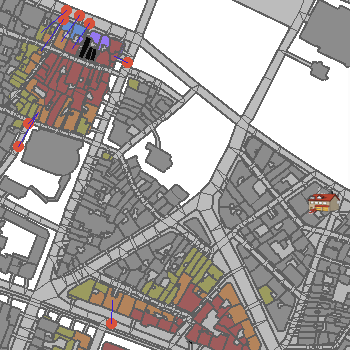
\includegraphics[width=.6\textwidth]{rcrs-detail}
    \caption[Detail of an example problem in the RCRS]{%
    Detail of an example RCRS problem on the Paris map. The red dots are fire brigades and
    the blue lines are their water jets. The colour of a building indicates its status:
    grey means no damage; yellow to red means on fire; blue to purple means that the fire
    has been extinguished, and black means that the building is burnt. The darker the
    colour, the greater the damage. On the centre-right is a fire station, to which the
    fire brigades return to refill. White regions indicate irrelevant areas, such as
    rivers or non-flammable properties.}
    \label{fig:rcrs}
\end{figure}

The RCRS is based on scenarios \cite{rcrsmanual}. A \emph{scenario} is a class of
problems, whose main parameter is the number of agents. In RMASBench there are $5$,
respectively with $15$, $21$, $27$, $33$ and $40$ fire brigades. Other settings are:
\begin{itemize}
    \item Agents are homogeneous, that is, they all have the same speed and water tank
        size;
    \item There are $3$ ignition points, and each scenario is replicated $30$ times. At
        each execution, a pseudo-random number generator influences the way the fires
        spread from ignition points to nearby buildings;
    \item To get a non-trivial number of fires, agents are added $25$ seconds after
        the start;
    \item Each simulation runs for a maximum of $5$ minutes, ending earlier if all fires
        have been extinguished;
    \item For each coalition $C$ and task $v$, we have that $u(C, v) = |C|$, which is a
        special case of superadditive characteristic function \cite[Section
        $2.1.2.2$]{chalkiadakis2011};
    \item Deadlines and workloads are randomly generated by the RCRS.
\end{itemize}
For each scenario and algorithm, we plot the average and standard deviation of:
\begin{enumerate}
    \item Problem completion time (Section \ref{sec:tests});
    \item The number of buildings that burned at least once, denoted by $b_{once}$;
    \item \emph{Score}, or the percentage of damage suffered by the city, where $100\%$
        means completely burnt. This is the main RCRS metric, defined on the total area of
        the city buildings and scenario-based parameters;
    \item Average CPU time\footnote{Based on an Intel Xeon E5-2670 processor (octa-core
        2.6 GHz with Hyper-Threading).} per problem time unit.
\end{enumerate}
We do not consider message-related metrics because agents do not communicate in S-CTS
(Section \ref{sec:s-cts}).

\subsection{Results}\label{sec:roboresults}

\begin{figure}[t]
    \centering
    \begin{adjustbox}{width=\textwidth}
        \begin{tikzpicture}
    \begin{groupplot}[%
            group style={group size=2 by 2, vertical sep=1.75cm, horizontal sep=1.75cm},
            grid=both,
            grid style={line width=.1pt, draw=gray!10},
            major grid style={line width=.2pt,draw=gray!50},
            minor tick num=5,
            ymin=0,
            xtick={15,21,27,33,40},
            legend style={/tikz/every even column/.append style={column sep=1em}, legend
            columns=-1,at={(0.35,2.55)}, anchor=north east},
            cycle list name=exotic3]

        \nextgroupplot[ymin=50,xlabel=Number of agents,ylabel=Problem completion time,
        title=(a)]

        % S-CTS
        \addplot+[error bars/.cd, y dir=both, y explicit,%
        error bar style = {thick}] coordinates {%
            (15, 167.97) +- (18.4, 18.4)
            (21, 162.14) +- (19.11, 19.11)
            (27, 130.94) +- (15.06, 15.06)
            (33, 97.94)  +- (10.38, 10.38)
            (40, 82.34)  +- (5.47, 5.47)
        };

        % DSA
        \addplot+[error bars/.cd, y dir=both, y explicit,%
        error bar style = {thick}] coordinates {%
            (15, 191.44) +- (19.7, 19.7)
            (21, 111.47) +- (13.98, 13.98)
            (27, 73.8)   +- (2.9, 2.9)
            (33, 65)     +- (1.39, 1.39)
            (40, 58.27)  +- (1.24, 1.24)
        };

        % BMS
        \addplot+[error bars/.cd, y dir=both, y explicit,%
        error bar style = {thick}] coordinates {%
            (15, 155.5) +- (19.04, 19.04)
            (21, 75.54) +- (3.95, 3.95)
            (27, 67.24) +- (1.35, 1.35)
            (33, 61.64) +- (0.64, 0.64)
            (40, 60.44) +- (1.09, 1.09)
        };

        \nextgroupplot[xlabel=Number of agents,ylabel=$b_{once}$, title=(b)]

        % S-CTS
        \addplot+[error bars/.cd, y dir=both, y explicit,%
        error bar style = {thick}] coordinates {%
            (15, 468.67) +- (105.57, 105.57)
            (21, 417.57) +- (96.05, 96.05)
            (27, 152.57) +- (48.29, 48.29)
            (33, 58.6) +- (18.42, 18.42)
            (40, 37.9) +- (5.34, 5.34)
        };

        % DSA
        \addplot+[error bars/.cd, y dir=both, y explicit,%
        error bar style = {thick}] coordinates {%
            (15, 587.1) +- (104.18, 104.18)
            (21, 186.54) +- (70.6, 70.6)
            (27, 32.87) +- (1.93, 1.93)
            (33, 29.64) +- (1.3, 1.3)
            (40, 26.54) +- (1.11, 1.11)
        };

        % BMS
        \addplot+[error bars/.cd, y dir=both, y explicit,%
        error bar style = {thick}] coordinates {%
            (15, 395.07) +- (98.67, 98.67)
            (21, 31.64) +- (2.77, 2.77)
            (27, 26.9) +- (0.83, 0.83)
            (33, 26) +- (0.8, 0.8)
            (40, 25.44) +- (0.84, 0.84)
        };

        \nextgroupplot[xlabel=Number of agents,ylabel=Score (\%), title=(b)]

        % S-CTS
        \addplot+[error bars/.cd, y dir=both, y explicit,%
        error bar style = {thick}] coordinates {%
            (15, 8.5108) +- (1.94, 1.94)
            (21, 9.86725) +- (2.27, 2.27)
            (27, 3.99635) +- (1.49, 1.49)
            (33, 1.43590) +- (0.31, 0.31)
            (40, 0.98847) +- (0.002, 0.002)
        };

        % DSA
        \addplot+[error bars/.cd, y dir=both, y explicit,%
        error bar style = {thick}] coordinates {%
            (15, 12.68) +- (2.375, 2.375)
            (21, 5.09) +- (1.93, 1.93)
            (27, 0.99) +- (0.0009, 0.0009)
            (33, 0.99175) +- (0.0004, 0.0004)
            (40, 0.99264) +- (0.0004, 0.0004)
        };

        % BMS
        \addplot+[error bars/.cd, y dir=both, y explicit,%
        error bar style = {thick}] coordinates {%
            (15, 6.63) +- (1.58, 1.58)
            (21, 0.99) +- (0.001, 0.001)
            (27, 0.99278) +- (0.0002, 0.0002)
            (33, 0.99325) +- (0.0001, 0.0001)
            (40, 0.99342) +- (0.0001, 0.0001)
        };

        \nextgroupplot[xlabel=Number of agents,ylabel=Average CPU time (ms), title=(d)]

        % S-CTS
        \addplot+[error bars/.cd, y dir=both, y explicit,%
        error bar style = {thick}] coordinates {%
            (15, 9.9) +- (1.76, 1.76)
            (21, 16.84) +- (3.44, 3.44)
            (27, 9.97) +- (2.465, 2.465)
            (33, 6.8) +- (0.68, 0.68)
            (40, 11.37) +- (0.57, 0.57)
        };

        % DSA
        \addplot+[error bars/.cd, y dir=both, y explicit,%
        error bar style = {thick}] coordinates {%
            (15, 24.54) +- (3.37, 3.37)
            (21, 19.97) +- (4.14, 4.14)
            (27, 17.57) +- (0.43, 0.43)
            (33, 23.1) +- (0.53, 0.53)
            (40, 44.34) +- (1.34, 1.34)
        };

        % BMS
        \addplot+[error bars/.cd, y dir=both, y explicit,%
        error bar style = {thick}] coordinates {%
            (15, 255.1) +- (44.11, 44.11)
            (21, 129.57) +- (4.87, 4.87)
            (27, 164.77) +- (3.4, 3.4)
            (33, 187.54) +- (7.14, 7.14)
            (40, 263.47) +- (6.63, 6.63)
        };

    \legend{\textsc{s-cts}, \textsc{dsa}, \textsc{binaryms}}
    \end{groupplot}
\end{tikzpicture}

    \end{adjustbox}
    \caption[Performance of S-CTS in RMASBench]{%
        Performance of S-CTS in RMASBench using DSA and Binary Max-Sum as baselines. In
        each figure, the X-axis defines the number of agents in the scenario, while each
        point is the $avg \pm std/2$, where $avg$ is the average over 30 simulations of
        the value indicated by the Y-axis, and $std$ is the standard deviation of $avg$.}
    \label{fig:c1test2}
\end{figure}

The more agents communicate with each other, the better they coordinate. In turn, this
leads to lower completion times and numbers of burned buildings. Because there is no
exchange of messages in S-CTS and BinaryMS has the highest communication overhead, they
are respectively the least and the most performing in Figures \ref{fig:c1test2}a and
\ref{fig:c1test2}b.
Nevertheless, this does not result in a drastic drop in performance. In Figure
\ref{fig:c1test2}c, in the worst-case scenario (i.e., $21$ agents), on average S-CTS
scores about $10\%$ (resp. $5\%$) less than BinaryMS (resp. DSA). This is not trivial,
given that S-CTS is a simplification and that the scenarios used are fine-tuned to
maximise the performance of BinaryMS and DSA.

Regarding the average CPU time (Figure \ref{fig:c1test2}d), S-CTS is up to two orders of
magnitude (resp. 1) faster than BinaryMS (resp. DSA). This is because BinaryMS has a
pre-processing phase that requires exponential time, while DSA, despite having a time
complexity similar to that of S-CTS (Table \ref{t:dcop_chars}), has a message-passing
phase as well.

In Figures \ref{fig:c1test2}a, \ref{fig:c1test2}b and \ref{fig:c1test2}c, the trends
converge to $0$ because the more agents there are, the less relevant the algorithm being
used becomes. In other words, the greater the number of available agents, the higher the
quality of solutions. We can deduce that the degree of agent communication is directly
proportional to the score and inversely proportional to the CPU time. However, as we have
seen, the difference in performance between communication and no communication is not
necessarily significant.

\section{Summary}

We presented CFLA2, a version of CFLA with a more detailed Phase $2$ and an improved Phase
$3$. Since we show that the time complexity of CFLA2 is quadratic in the number of tasks
and exponential in the number of agents, and that the look-ahead technique cannot be
used in dynamic environments, we also presented CTS, the first anytime and efficient
CFSTP algorithm with convergence guarantee. We demonstrated the superiority of CTS in
settings that largely favour the look-ahead technique, and showed that a simplified but
parallel variant is enough to compete with high-performance baselines in the RCRS,
at a fraction of their time complexity.
The next chapter extends CTS to large-scale dynamic and distributed environments, which
fall within our research objectives (Section \ref{sec:objectives}).
